\documentclass[letterpaper,12pt]{article}
\usepackage{array}
\usepackage{threeparttable}
\usepackage{geometry}
\usepackage{float}
\geometry{letterpaper,tmargin=1in,bmargin=1in,lmargin=1.25in,rmargin=1.25in}
\usepackage{fancyhdr,lastpage}
\pagestyle{fancy}
\lhead{}
\chead{}
\rhead{}
\lfoot{}
\cfoot{}
\rfoot{\footnotesize\textsl{Page \thepage\ of \pageref{LastPage}}}
\renewcommand\headrulewidth{0pt}
\renewcommand\footrulewidth{0pt}
\usepackage[format=hang,font=normalsize,labelfont=bf]{caption}
\usepackage{listings}
\lstset{frame=single,
  language=Python,
  showstringspaces=false,
  columns=flexible,
  basicstyle={\small\ttfamily},
  numbers=none,
  breaklines=true,
  breakatwhitespace=true
  tabsize=3
}
\usepackage{amsmath}
\usepackage{amssymb}
\usepackage{amsthm}
\usepackage{harvard}
\usepackage{setspace}
\usepackage{float,color}
\usepackage[pdftex]{graphicx}
\usepackage{hyperref}
\hypersetup{colorlinks,linkcolor=red,urlcolor=blue}
\theoremstyle{definition}
\newtheorem{theorem}{Theorem}
\newtheorem{acknowledgement}[theorem]{Acknowledgement}
\newtheorem{algorithm}[theorem]{Algorithm}
\newtheorem{axiom}[theorem]{Axiom}
\newtheorem{case}[theorem]{Case}
\newtheorem{claim}[theorem]{Claim}
\newtheorem{conclusion}[theorem]{Conclusion}
\newtheorem{condition}[theorem]{Condition}
\newtheorem{conjecture}[theorem]{Conjecture}
\newtheorem{corollary}[theorem]{Corollary}
\newtheorem{criterion}[theorem]{Criterion}
\newtheorem{definition}[theorem]{Definition}
\newtheorem{derivation}{Derivation} % Number derivations on their own
\newtheorem{example}[theorem]{Example}
\newtheorem{exercise}[theorem]{Exercise}
\newtheorem{lemma}[theorem]{Lemma}
\newtheorem{notation}[theorem]{Notation}
\newtheorem{problem}[theorem]{Problem}
\newtheorem{proposition}{Proposition} % Number propositions on their own
\newtheorem{remark}[theorem]{Remark}
\newtheorem{solution}[theorem]{Solution}
\newtheorem{summary}[theorem]{Summary}
%\numberwithin{equation}{section}
\bibliographystyle{aer}
\newcommand\ve{\varepsilon}
\newcommand\boldline{\arrayrulewidth{1pt}\hline}
\graphicspath{{images/}}


\begin{document}

\begin{flushleft}
  \textbf{\large{Problem Set \#4}} \\
  MACS 30100, Dr. Evans \\
  Ningyin Xu
\end{flushleft}

\vspace{5mm}

\noindent\textbf{Problem 1. Some income data, lognormal distribution, and MM.}
\\
\noindent\textbf{Part (a).} \\
\\
\begin{figure}[htb]\centering\captionsetup{width=4.0in}
  \label{Fig1a}
  \fbox{\resizebox{4.0in}{3.0in}{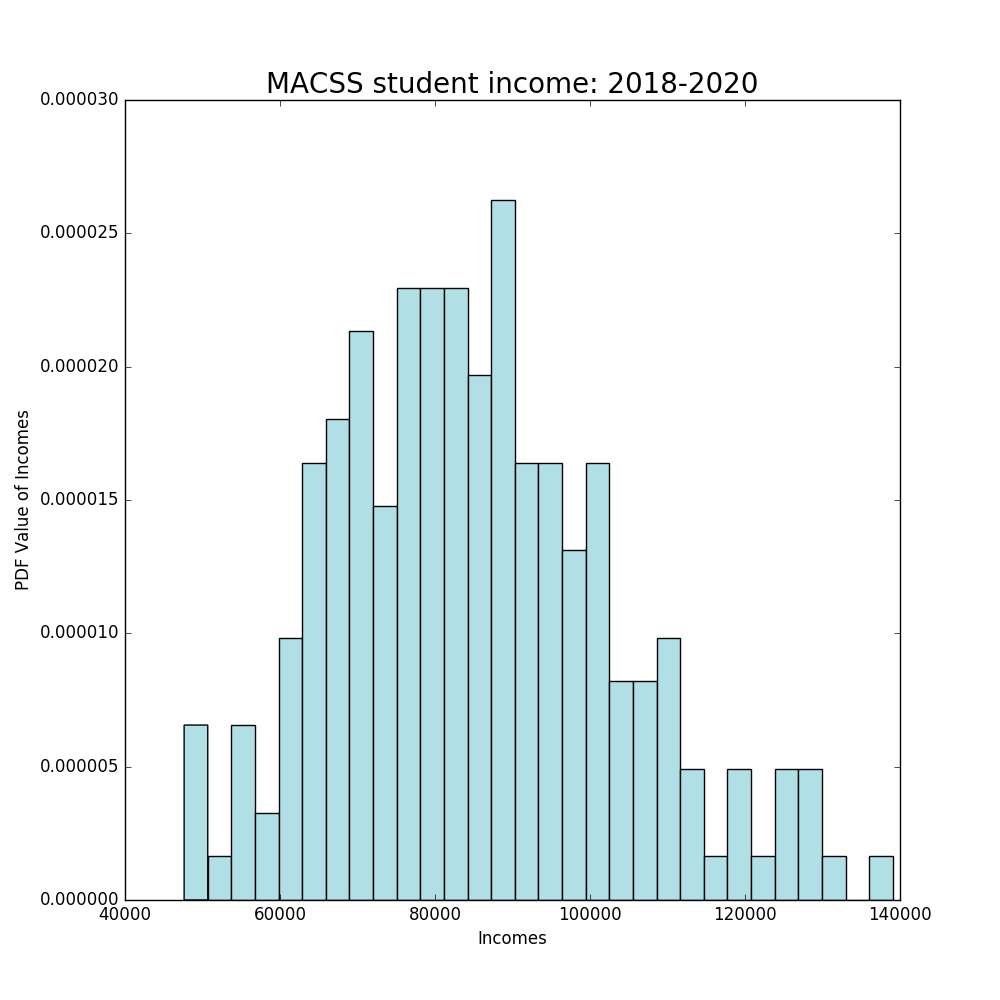
\includegraphics{Fig_1a.png}}}
\end{figure}
\\
\noindent\textbf{Part (b).} \\
\\
The array returned from my LNpdf() functions is shown as below. It has the same size as the xvals, so the LNpdf() function is constructed successfully.\\
\\
$
\begin{bmatrix}
 0.0019079&  0.00123533 \\ 
 0.00217547&  0.0019646 \\  
\end{bmatrix}
$
\\
\newpage
\noindent\textbf{Part (c).}\\
\begin{figure}[htb]\centering\captionsetup{width=4.0in}
  \label{Fig1c}
  \fbox{\resizebox{4.0in}{3.0in}{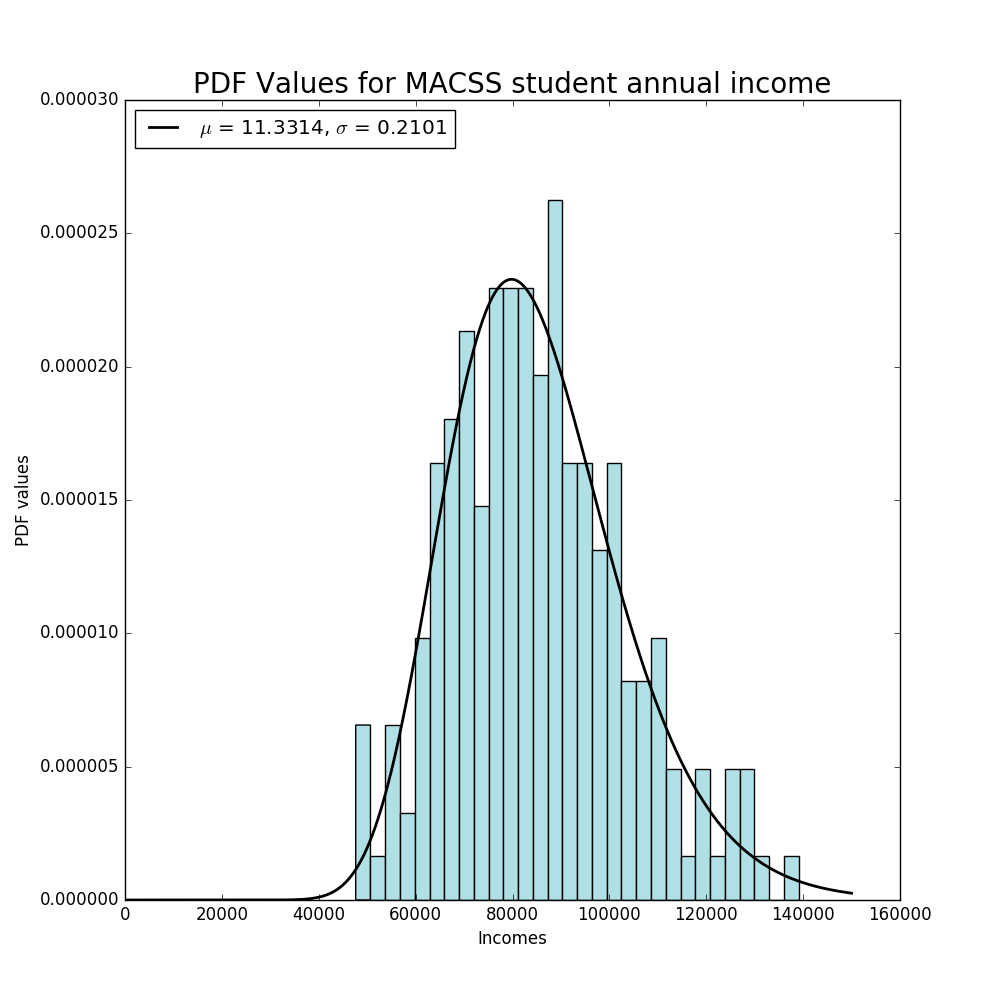
\includegraphics{Fig_1c.png}}}
\end{figure}
\\
The value of SMM criterion function at the estimated parameter values is: \\
$9.826886786295898e-14$.\\
And the data moments are: $\mu = 85276.8236$, $\sigma = 17992.5421$.\\
Model moments at the estimated parameter values are: $\mu = 85276.8173$, $\sigma = 17992.5366$.\\
These model moments are very close to data moments, which means SMM estimation performs well.\\

\noindent\textbf{Part (d).}
\begin{figure}[htb]\centering\captionsetup{width=4.0in}
  \label{Fig1d}
  \fbox{\resizebox{4.0in}{3.0in}{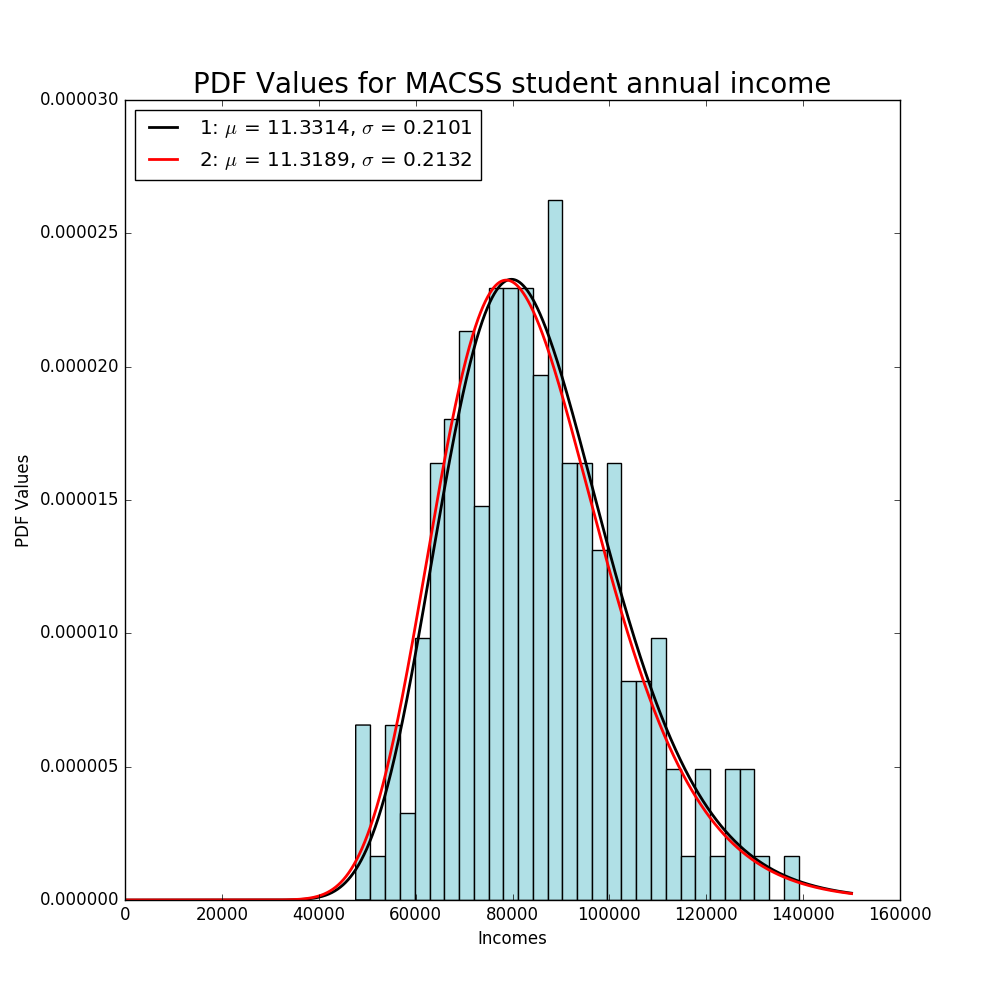
\includegraphics{Fig_1d.png}}}
\end{figure}

The value of GMM criterion function at the estimated parameter values is: \\
$0.04829947380858357$.\\
And the data moments are: $\mu = 85276.8236$, $\sigma = 17992.5421$.\\
Model moments at the estimated parameter values are: $\mu = 84273.1688$, $\sigma = 18043.5879$.\\
These model moments are also very close to data moments, which means 2-step SMM estimation performs well.\\


\end{document}
